\section{System architecture}

This section presents an overview of the architecture of the whole system. The system is decomposed into several Nodes. Together with the  RatSLAMRos and simulator, the system uses three custom nodes: Data fusion, LV Builder, and LV matching. Furthermore, the system contains two additional nodes that do not influence the algorithm's run but are used for the performance analyses and other help utilities, helping with the development process. The system architecture is presented in Figure \ref{fig:systemArchitecture}. The visualization and topics used only for visualization purposes are omitted for clarity.

\begin{figure}[htpb]
    \centering
    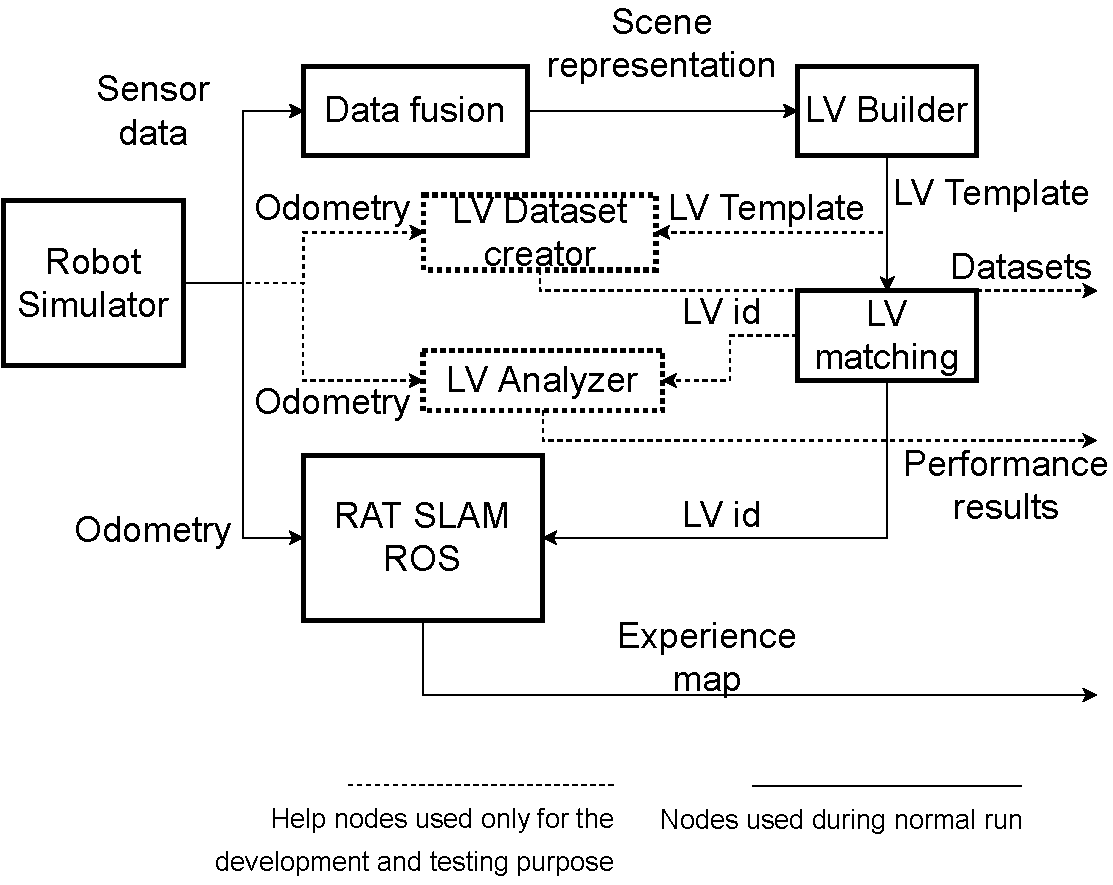
\includegraphics[width=0.8\textwidth]{systemArchitecture.pdf}
    \caption{Diagram of the ROS nodes in the whole system} \label{fig:systemArchitecture}
\end{figure}

\subsection{Robot Simulator}

This node represents the whole simulation and can be easily replaced with a physical robot. The robot is simulated using a Gazebo simulator, introduced in chapter [TODO chapter ref]. Besides much other information about the scene and the robot, the simulation publishes data from sensors, namely HD Camera and 3D LiDAR, and odometry data, further consumed by other nodes.

% TODO check topic names
\begin{table}[htpb]
    \caption{Relevant topics published by the simulator}\label{tab:robotSimulatorTopics}
    \centering
    \begin{tabular}{l l l}
        \toprule
        Topic                   & Type                          & Mode    \\
        \midrule
        camera/rgb/camera\_info & sensor\_msgs::CameraInfo      & publish \\
        camera/rgb/image\_raw   & sensor\_msgs::CompressedImage & publish \\
        velodyne\_points        & sensor\_msgs::PointCloud2     & publish \\
        odom                    & nav\_msgs::Odometry           & publish \\
        \bottomrule
    \end{tabular}
\end{table}

\subsection{Data fusion}

The goal of this node is to take raw data from the sensors and create a single representation of the environment, combining the advantages of each sensor. This node takes care of the synchronization of the sensors, dealing with different frames of reference and the fusion itself. The data fusion node subscribes to the camera and LiDAR topics published by simulation or a real robot and publishes one topic with the final environment representation. How this node exactly works is described in the section [TODO chapter ref].

% TODO check topic names
\begin{table}[htpb]
    \caption{Subscribed and published topics by the Data fusion node}\label{tab:dataFusionTopics}
    \centering
    \begin{tabular}{l l l}
        \toprule
        Topic                   & Type                          & Mode      \\
        \midrule
        camera/rgb/camera\_info & sensor\_msgs::CameraInfo      & subscribe \\
        camera/rgb/image\_raw   & sensor\_msgs::CompressedImage & subscribe \\
        velodyne\_points        & sensor\_msgs::PointCloud2     & subscribe \\
        rgb\_cloud              & sensor\_msgs::PointCloud2     & publish   \\
        \bottomrule
    \end{tabular}
\end{table}

\subsection{LV Builder}

This node subscribes single topic published by the Data Fusion node. The main task of this node is to take the environment representation and reformat it into a suitable template that will be stored in a memory and compared with previously visited scenes. This node publishes a topic with the built template and two other topics for visualization and debugging purposes. Three different approaches to the exact implementation of this node are described in the sections [TODO chapters ref].

% TODO check topic names
\begin{table}[htpb]
    \caption{Subscribed and published topics by the LV Builder node}\label{tab:lvBuilderTopics}
    \centering
    \begin{tabular}{l l l}
        \toprule
        Topic                      & Type                                                                                              & Mode      \\
        \midrule
        rgb\_cloud                 & sensor\_msgs::PointCloud2                                                                         & subscribe \\
        current\_scene\_descripion & msgs::LVDescription\tablefootnote{Self defined message, see [TODO msg description and reference]} & publish   \\
        clustered\_viz             & sensor\_msgs::PointCloud2                                                                         & publish   \\
        convex\_hull\_viz          & sensor\_msgs::PointCloud2                                                                         & publish   \\
        \bottomrule
    \end{tabular}
\end{table}
\subsection{LV Matching}

This node subscribes to a topic published by the LV Builder node. The goal of this node is to store all visited places, assign unique ids to all seen scenes, compare a received scene with other scenes, and decide if it was already seen. If the currently received scene template is similar enough to some of the stored templates, this node publishes the id of the matched template. If there is no such template, this node generates and publishes a brand new id and stores the received template as a newly visited place. The only topic this node is publishing is a topic with ids of matched or new scenes.

% TODO check topic names
\begin{table}[htpb]
    \caption{Subscribed and published topics by the LV Matching node}\label{tab:lvMatchingTopics}
    \centering
    \begin{tabular}{l l l}
        \toprule
        Topic                      & Type                       & Mode      \\
        \midrule
        current\_scene\_descripion & msgs::LVDescription        & subscribe \\
        LocalView/Template         & ratslam\_ros::ViewTemplate & publish   \\
        \bottomrule
    \end{tabular}
\end{table}

\subsection{Rat SLAM Ros}

This diagram block represents not a single node but a whole package from several nodes. This is an original RatSLAMRos described in chapter [TODO chapter ref], run without almost any changes. The only difference compared to the original package is the number of started nodes. The lv Node is not activated because its job is done by LV Builder and LV Matching node, and the visual odometry Node is replaced by an odometry sensor from the simulator. The package subscribes to the topic with scene ids published by the LV matching node and to the topic with odometry directly from the simulator. The only relevant published topic is the experience map topic, with the final experience map, which is the final result of the whole algorithm.

% TODO check topic names
\begin{table}[htpb]
    \caption{Relevant subscribed and published topics by the RatSLAMRos package}\label{tab:ratslamTopics}
    \centering
    \begin{tabular}{l l l}
        \toprule
        Topic              & Type                         & Mode      \\
        \midrule
        LocalView/Template & ratslam\_ros::ViewTemplate   & subscribe \\
        odom               & nav\_msgs::Odometry          & subscribe \\
        ExperienceMap/Map  & ratslam\_ros::TopologicalMap & publish   \\
        \bottomrule
    \end{tabular}
\end{table}

\subsection{LV Analyzer}

This node subscribes to the same topics as the Rat SLAM Ros package. This node serves only debugging purposes and does not influence the algorithm. The goal of this node is to evaluate the performance of the algorithm. It receives all the ids of matched and new ids from the LV Matching node and can pair them with the exact position of the robot at the time the scene template was taken because of the information received from the simulator. This node remembers the precise position of each scene newly remembered by the LV Matching node and can calculate the position difference between each match and the original matched scene. Furthermore, it can calculate the distance to the nearest previously visited scene for each newly added template. According to the metrics described in the section [TODO section ref], the number of false positive and false negative matches can be calculated, leading to the approach's final accuracy, recall, and precision. These estimated numbers are the final output of this node.


% TODO check topic names
\begin{table}[htpb]
    \caption{Subscribed  topics by the LV Analyzer node}\label{tab:lvAnalTopics}
    \centering
    \begin{tabular}{l l l}
        \toprule
        Topic                 & Type                          & Mode      \\
        \midrule
        LocalView/Template    & ratslam\_ros::ViewTemplate    & subscribe \\
        odom                  & nav\_msgs::Odometry           & subscribe \\
        camera/rgb/image\_raw & sensor\_msgs::CompressedImage & subscribe \\
        \bottomrule
    \end{tabular}
\end{table}

\subsection{LV Dataset creator}

This node works in principle similar to the LV Analyzer node. The goal of this node is to pair the templates with their exact positions received from the simulator. Unlike the LV Analyzer node, this node receives and pairs the whole template from the LV Builder node instead of only the scene id from the LV Matching node. The set of pairs of templates and their exact positions is the output of this node, which helps build final datasets for automatic parameter tuning, see chapter [TODO chapter ref], or neural networks training, see chapter [TODO chapter ref].


% TODO check topic names
\begin{table}[htpb]
    \caption{Subscribed  topics by the Dataset creator node}\label{tab:datasetCreatorTopics}
    \centering
    \begin{tabular}{l l l}
        \toprule
        Topic                      & Type                & Mode      \\
        \midrule
        current\_scene\_descripion & msgs::LVDescription & subscribe \\
        odom                       & nav\_msgs::Odometry & subscribe \\
        \bottomrule
    \end{tabular}
\end{table}